\subsection{Hardware design}
\label{sec:des-hardware}
The hardware must hold the paper and pen securely, reach the required writing area, and convert a stored trajectory into repeatable motion. The design therefore combines a Cartesian belt drive with a separately actuated pen mechanism. The electrical interface is kept simple enough for direct control from the ODROID, while calibration relates software coordinates to the travel of the assembled machine.

\subsubsection{Plotter designs and mechanics}
The chosen method of text plotting is a Cartesian gantry system with two independent axes of movement and a pen up/down mechanism, consistent with the Cartesian arrangement illustrated by Teikari~\cite[p.~6]{teikari2016}. Complex kinematic equations and joint-dependent position errors are avoided by using separate $x$ and $y$ movements for reproduction. Linear GT2 timing belts and pulleys are used to convert rotary motion from stepper motors and axles to the desired Cartesian movements. Timing belts were chosen for their cost effectiveness and ability to provide relatively fast travel without a lead-screw transmission.

A Cartesian gantry consists of stationary rails that guide movement in one axis, and a movable rail that guides the other axis of movement. For this system and the explanations that follow, the stationary rails guide $y$-axis movement, while the $x$-axis rail moves along the $y$-axis. Figure~\ref{fig:des-gantry-axes} shows the axes of the gantry.

\begin{figure}[!htbp]\centering
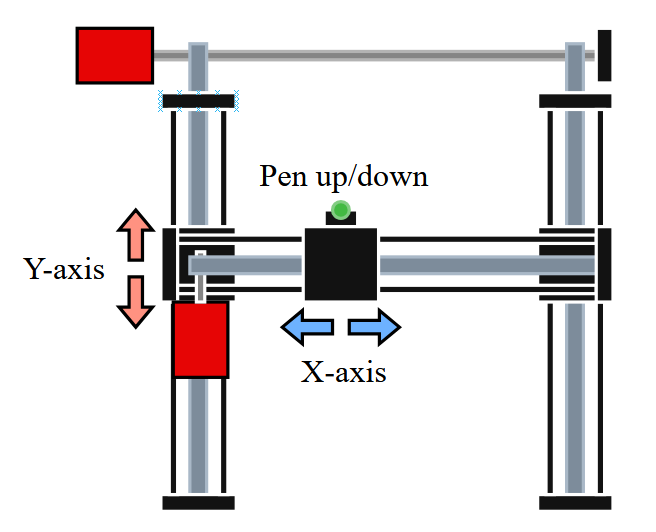
\includegraphics[width=0.67\linewidth]{Figures/gantry-axis-diagram.png}
\caption{Cartesian gantry axes and pen up/down mechanism.}
\label{fig:des-gantry-axes}
\end{figure}

The $x$-axis rail needs to move with stability and consistency, which is why it is supported at both ends by the two $y$-axis rails. A single stepper motor was chosen to drive the pulleys on both sides to ensure synchronised motion and save costs. Two independent stepper motors driving one axis introduce a synchronisation concern because differences in missed steps or loading could offset one side relative to the other. The challenge with using one motor to drive two timing pulleys is extending its shaft to both pulleys without excessive load or twist in the new axle. A rigid coupler was used to extend the stepper motor shaft with a chromed steel rod.

To reduce strain on the motors and allow smoother movement, linear bearings were fitted around the chromed rod rails so that the moving parts slide with low resistance. Bearing alignment is important as well as bearing diameter, because an incorrectly aligned bearing can constrain the same rod in a different direction from the neighbouring bearing, increasing resistance instead of reducing it. During construction of the gantry, bearing alignment was checked by fitting the bearing in its respective support part and sliding it along the rails to ensure minimal friction before connecting the belts.

The CAD components in Figure~\ref{fig:gantry-cad-components} position the rods, bearings, pulleys, switches and pen mechanism. Designing these supports together allowed their mounting positions and clearances to suit the assembled gantry. The bearing supports were checked on the rods before the belts were attached, so resistance from a tight or misaligned support could be corrected separately from belt tension.

\begin{figure}[!htbp]
    \centering
    \begin{minipage}[c]{0.48\linewidth}
        \centering
        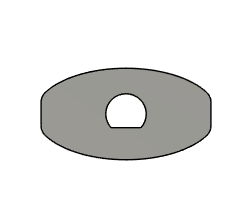
\includegraphics[width=\linewidth,height=0.16\textheight,keepaspectratio]{Figures/cad-component-01.png}
    \end{minipage}\hfill
    \begin{minipage}[c]{0.48\linewidth}
        \centering
        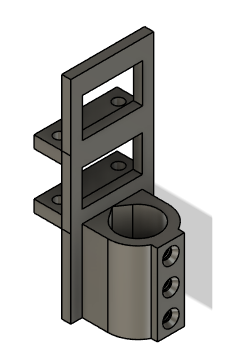
\includegraphics[width=\linewidth,height=0.16\textheight,keepaspectratio]{Figures/cad-component-02.png}
    \end{minipage}\\[0.5em]
    \begin{minipage}[c]{0.48\linewidth}
        \centering
        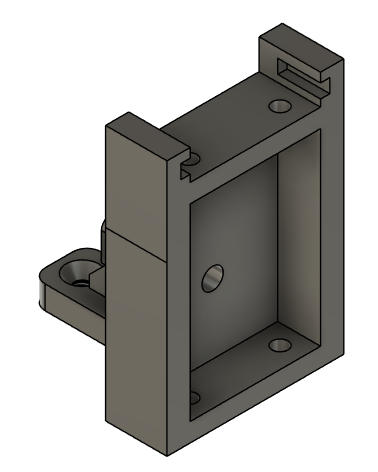
\includegraphics[width=\linewidth,height=0.16\textheight,keepaspectratio]{Figures/cad-component-03.png}
    \end{minipage}\hfill
    \begin{minipage}[c]{0.48\linewidth}
        \centering
        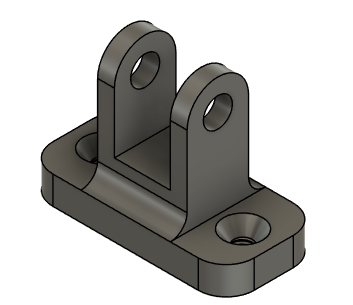
\includegraphics[width=\linewidth,height=0.16\textheight,keepaspectratio]{Figures/cad-component-04.png}
    \end{minipage}\\[0.5em]
    \begin{minipage}[c]{0.48\linewidth}
        \centering
        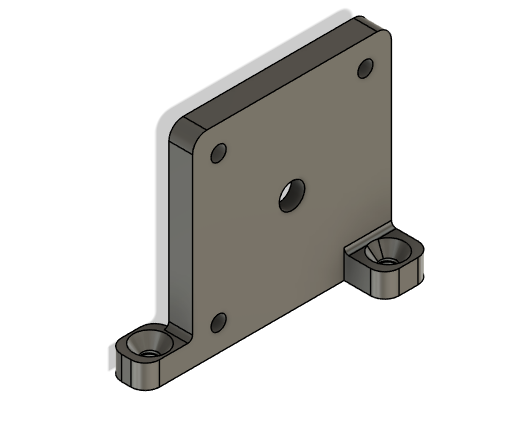
\includegraphics[width=\linewidth,height=0.16\textheight,keepaspectratio]{Figures/cad-component-05.png}
    \end{minipage}\hfill
    \begin{minipage}[c]{0.48\linewidth}
        \centering
        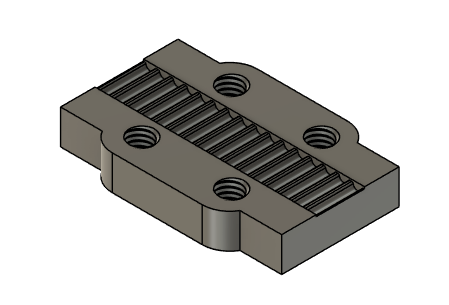
\includegraphics[width=\linewidth,height=0.16\textheight,keepaspectratio]{Figures/cad-component-06.png}
    \end{minipage}\\[0.5em]
    \begin{minipage}[c]{0.48\linewidth}
        \centering
        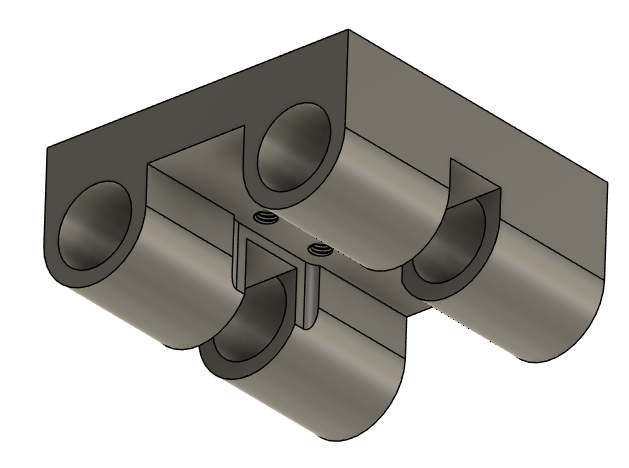
\includegraphics[width=\linewidth,height=0.16\textheight,keepaspectratio]{Figures/cad-component-07.png}
    \end{minipage}\hfill
    \begin{minipage}[c]{0.48\linewidth}
        \centering
        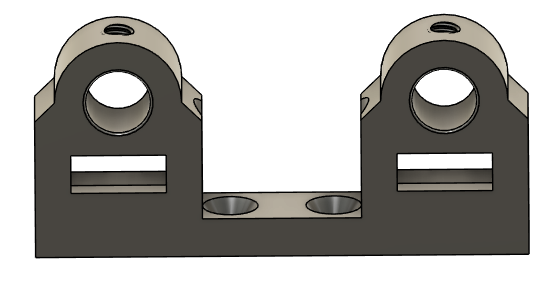
\includegraphics[width=\linewidth,height=0.16\textheight,keepaspectratio]{Figures/cad-component-08.png}
    \end{minipage}
    \caption{CAD models of the gantry components.}
    \label{fig:gantry-cad-components}
\end{figure}

\label{sec:des-camera}
The camera and page restraint provide the input to the recognition system. An IMX179 USB autofocus webcam is positioned over the secured page; the captured image follows the same processing path as an uploaded image. Its advertised 8\,MP resolution does not establish the resolution negotiated by the capture software.

\subsubsection{Stepper motor and driver}
\label{sec:des-stepper}
A stepper motor turns through fixed angular increments as the winding-current pattern changes. The A4988 regulates these winding currents by chopping: it switches the drive to maintain the desired current level. Chopping continues even while a position is held and the motor is not rotating. The a step is induced by changing the current pattern, chopping occurs at high frequencies regardless of the steps.~\cite[p.~9]{a4988ds}.

Two stepper motors are used in the gantry plotter, one for the $x$ and one for the $y$ direction. The selected motor is the 42BYGH40-01 NEMA 17 bipolar stepper, with a 40\,mm body length, a $1.8^\circ$ full-step angle and a rated current of 1.68\,A per phase. Stepper motors are ideal for precise gantry movement, because they produce movement and rotations at specific, consistent intervals, and hold in the same position even when the motors are not moving. Encoders are not used in this design: position is tracked through the commanded steps, which assumes the motors do not miss steps~\cite{acarnley2002}.

\label{sec:des-power}
Each motor is controlled by an A4988 driver supplied from the 24\,V supply, with 3.3\,V logic and STEP/DIR signals from the ODROID. The supply limit of 2.11\,A is separate from the driver's phase-current limit. The latter is set by the reference voltage and sense resistance~\cite[p.~9]{a4988ds}:
\begin{equation}
I_{\mathrm{trip,max}}=\frac{V_{\mathrm{ref}}}{8R_S}.
\label{eq:des-current}
\end{equation}
For the reported R10 marking, $R_S=0.10\,\Omega$ gives a reference-voltage ceiling of $8(0.10)(1.68)=1.344$\,V at the motor's rated phase current. This is a rating-based ceiling, not a measured driver setting; carrier heating can require a lower current. The detailed pin and supply connections remain in Table~\ref{tab:des-pin-map} in the appendix.

\paragraph{Speed-to-torque margin check.}
The following calculations retain the original sizing check for one motor driving the 950\,g moving assembly. Dziedzic et al. studied handwritten samples produced at 10--60\,mm/s~\cite{dziedzic2026}. The upper value provides the original speed benchmark: $60(60)=3600$\,mm/min, rounded upwards to 4000\,mm/min for the motor-sizing check. This is design headroom, rather than the selected drawing feed. The current generated jobs use 900\,mm/min for drawing and 2400\,mm/min for travel.

The installed 20-tooth GT2 pulley advances the belt by $20(2)=40$\,mm per revolution. Converting the design feed to shaft speed gives~\cite{acarnley2002}
\begin{equation}
n=\frac{F}{\ell_{\mathrm{rev}}}
=\frac{4000\ \mathrm{mm/min}}{40\ \mathrm{mm/rev}}
=100\ \mathrm{rev/min}.
\label{eq:gan-rpm}
\end{equation}
At the selected travel and drawing feeds, the corresponding speeds are $2400/40=60$\,rev/min and $900/40=22.5$\,rev/min. The torque comparison is therefore made at the higher 100\,rev/min sizing point, rather than using holding torque alone.

The original check used the curve points $(n_1,T_1)=(60\,\mathrm{rev/min},7\,\mathrm{N\,cm})$ and $(n_2,T_2)=(120\,\mathrm{rev/min},21\,\mathrm{N\,cm})$. Retaining those earlier curve readings provisionally, linear interpolation gives
\begin{equation}
T_{\mathrm{po}}(100)=T_1+\frac{100-n_1}{n_2-n_1}(T_2-T_1)
=7+\frac{100-60}{120-60}(21-7)
=16.33\ \mathrm{N\,cm}.
\label{eq:gan-pullout}
\end{equation}
The matching motor, supply and phase-current conditions for these curve readings are not established in the retained source record. Consequently, this is a conditional sizing value, rather than a verified pull-out torque for the installed motor.

The bearings support the moving assembly, so the motor moves its 950\,g mass horizontally rather than lifting its full weight. Retaining the original assumed rolling-friction coefficient $\mu=0.004$, the steady-speed load follows from $F_f=\mu mg$ and $T=r_pF_f$~\cite{acarnley2002}. The correct GT2 pitch radius is $r_p=20(0.002)/(2\pi)=0.006366$\,m, giving
\begin{equation}
T_{\mathrm{req}}=r_p\mu mg
=0.006366(0.004)(0.950)(9.81)
=2.37\times10^{-4}\ \mathrm{N\,m}
=0.0237\ \mathrm{N\,cm}.
\label{eq:des-torque}
\label{eq:gan-treq}
\end{equation}
Here the 950\,g is the complete moving load; supporting it on two rails does not double its mass. The resulting conditional torque ratio is
\begin{equation}
\frac{T_{\mathrm{po}}}{T_{\mathrm{req}}}
=\frac{16.33}{0.02373}\approx688.
\label{eq:gan-margin}
\end{equation}
This reproduces the reasoning behind choosing one motor and a shared shaft for the two belt drives: under the assumed bearing resistance and earlier curve values, the steady-speed load is small compared with the available torque estimate. The ratio is not a measured safety factor. It excludes acceleration, belt preload, shaft and bearing misalignment, and depends on the applicability of the earlier torque curve. It therefore supports the original sizing argument without establishing that every starting rate is safe.

\begin{figure}[!htbp]\centering
\begin{minipage}{0.48\linewidth}\centering
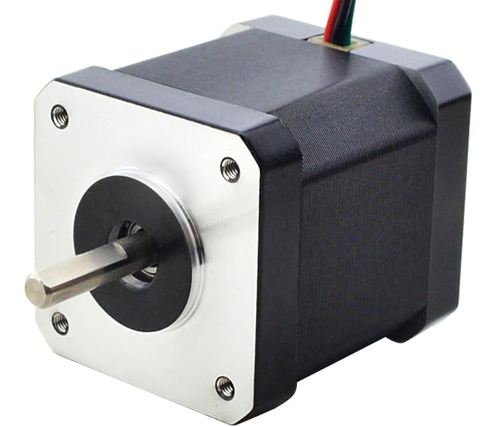
\includegraphics[width=\linewidth,height=0.18\textheight,keepaspectratio]{Figures/nema-17-stepper-motor.png}
\end{minipage}\hfill
\begin{minipage}{0.48\linewidth}\centering
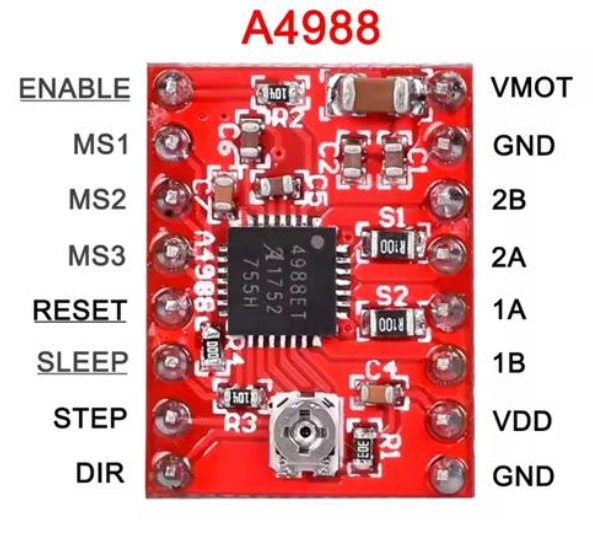
\includegraphics[width=\linewidth,height=0.18\textheight,keepaspectratio]{Figures/a4988-stepper-driver.png}
\end{minipage}
\caption{NEMA 17 stepper motor and A4988 driver used in the gantry.}
\label{fig:stepper-motor-and-driver}
\end{figure}

\subsubsection{Step resolution, microstepping and calibration}
Using the stepper transmission relationship~\cite{acarnley2002}, Equation~\ref{eq:des-pulley} derives the travel per revolution $\ell_{\mathrm{rev}}$ and pitch radius $r_p$for the installed 20-tooth GT2 pulleys and 2mm belt pitch.

\begin{equation}
\ell_{\mathrm{rev}}=N_t p=20(2)=40\ \mathrm{mm/rev},\qquad
r_p=\frac{N_t p}{2\pi}=6.37\ \mathrm{mm}.
\label{eq:des-pulley}
\end{equation}

$N_t$ refers to the tooth count and $p$ is belt pitch. The A4988 stepper motor driver allows substeps of $\mu_s=16$~\cite[p.~6]{a4988ds}. Combining this with 200 full steps per revolution gives the total distance in Equation~\ref{eq:des-stepres}.

\begin{equation}
\kappa_0=\frac{200\mu_s}{\ell_{\mathrm{rev}}}=80\ \mathrm{microsteps/mm},\qquad
\Delta x_0=\frac{1}{\kappa_0}=0.0125\ \mathrm{mm}.
\label{eq:des-stepres}
\end{equation}

The value in Equation~\ref{eq:des-stepres} is alot smaller than the proposal's 0.5mm positional-error limit. This means the stepper motors can produce fine enough rotation steps to meet the positional accuracy but there are many other hardware and software inconsistencies that could contrubute to final mm error.

This is the nominal command resolution. Calibration replaces the nominal steps per millimetre with the scale obtained from the assembled axes, as described below; it does not remove belt compliance or detect missed steps.

\subsubsection{Pen up/down mechanism}
\label{sec:des-pen}
A geared motor turns a cam to raise and lower the pen, as shown in Figure~\ref{fig:des-penmechanism}. This gives the two required positions without a third positioning axis. The pen holder restrains lateral movement, while a switch indicates the raised position. The motor turns in one direction and successive cam positions alternate between pen up and pen down.

\begin{figure}[!htbp]\centering
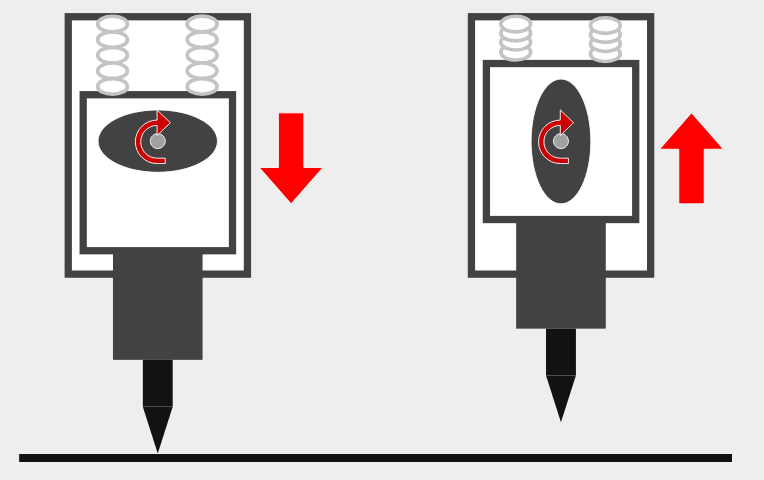
\includegraphics[width=0.66\linewidth]{Figures/pen-up-down-mechanism.png}
\caption{Cam-operated mechanism with the pen lowered and raised.}
\label{fig:des-penmechanism}
\end{figure}

A BC337 transistor switches the motor current, while the GPIO supplies the base-control signal through a 1\,k$\Omega$ resistor. The motor supply comes from the ODROID's dedicated 3.3\,V rail rather than a GPIO signal pin. Using the base-resistor relationship~\cite{rohmlowside2026}, with an assumed $V_{BE}=0.7$\,V,
\begin{equation}
I_B=\frac{V_{\mathrm{GPIO}}-V_{BE}}{R_B}
=\frac{3.3-0.7}{1000}=2.6\ \mathrm{mA}.
\label{eq:des-basecurrent}
\end{equation}
This is the nominal base current; motor startup current is also needed to verify transistor saturation~\cite{bc337ds}. No flyback diode is fitted in the prototype. Adding one across the motor would limit the switching transient when its inductive current is interrupted~\cite{rohmlowside2026}.

\begin{figure}[!htbp]\centering
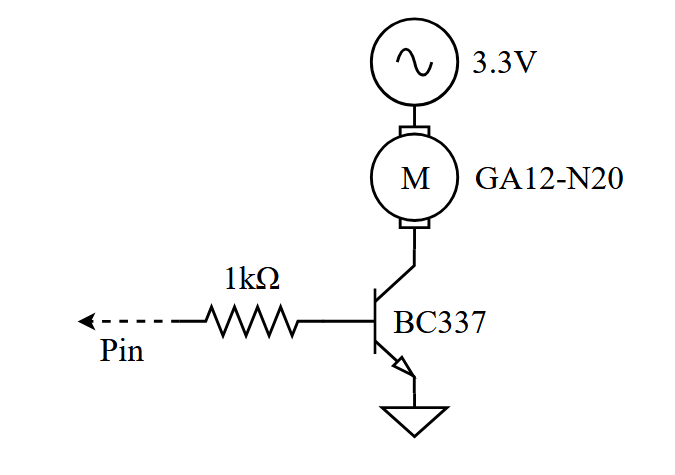
\includegraphics[width=0.60\linewidth]{Figures/pen-clicker-bc337-circuit.png}
\caption{Prototype BC337 pen-motor switching circuit.}
\label{fig:des-pencircuit}
\end{figure}

Before moving the pen, the controller checks its switch state to avoid an unnecessary rotation. It then runs the motor until the requested state is confirmed or the timeout expires, with a 40\,ms overrun after pen-up confirmation to seat the cam. The G-code file can request an additional settling dwell after changing pen state.

\subsubsection{End stop switches and calibration}
\label{sec:des-calibration}
Four switches mark the ends of the two axes, and a fifth switch indicates the pen state. The axis switches use active-high 3.3\,V inputs with 10\,k$\Omega$ pull-down resistors, as shown in Figure~\ref{fig:des-switch}. The pull-down holds the input low when the contact is open. Applying Ohm's law gives a closed-contact resistor current of $I=3.3/10000=0.33$\,mA and dissipation $P=3.3^2/10000=1.09$\,mW. A high input is accepted after three consecutive readings, 6\,ms apart, to reject brief switching noise and contact bounce.

\begin{figure}[!htbp]\centering
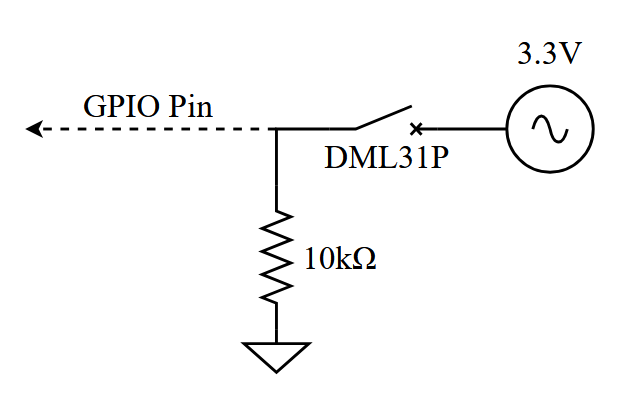
\includegraphics[width=0.62\linewidth]{Figures/endstop-switch-pulldown-circuit.png}
\caption{Active-high switch input with a 10\,k$\Omega$ pull-down.}
\label{fig:des-switch}
\end{figure}

Calibration moves each axis between its switches and counts the microsteps over the independently measured travel. These counts set the scale used for subsequent movement:
\begin{equation}
\kappa_x=\frac{N_x}{L_x},\qquad
\kappa_y=\frac{N_y}{L_y},\qquad
n_x=\operatorname{round}[(x+e)\kappa_x].
\label{eq:des-calibration}
\end{equation}
Here $N$ is the counted microsteps, $L$ is the measured switch-to-switch distance and $e=5$\,mm is the clearance from the end stop. The same expression applies to $y$. The configured travels of 200.6 and 261.3\,mm leave $200.6-2(5)=190.6$\,mm and $261.3-2(5)=251.3$\,mm of usable movement before writing margins. The measured calibration counts are required for numerical calibrated scales; 80 microsteps/mm remains the nominal value.

After calibration, the axes retract from the switches and the controller tracks position through signed step counts. Calibration is repeated after a restart. An end-stop event during drawing invokes the stop routine; the switches establish travel boundaries, rather than measuring continuous pen position.

\subsubsection{Gcode generation and motion mapping}
\label{sec:des-drive}
\label{sec:des-gcode-reading}
G-code describes a path as movement instructions, allowing a generated trajectory to be passed to the motor controller~\cite[p.~21]{teikari2016}. The reproduction stage creates this file; the hardware controller reads it line by line, extracts the command and its parameters, and converts target coordinates into axis movements. Table~\ref{tab:des-gcode-commands} summarises the subset used in the square-and-triangle job.

\begin{table}[!htbp]\centering\small
\begin{tabularx}{\linewidth}{|l|X|}\hline
\textbf{Command or parameter}&\textbf{Meaning in this plotter}\\\hline
\texttt{G21}, \texttt{G90}&Millimetre coordinates and absolute positioning.\\\hline
\texttt{G0}, \texttt{G1}&Travel and drawing moves, respectively; both use the linear-movement routine. Pen state is controlled separately.\\\hline
\texttt{X}, \texttt{Y}, \texttt{F}&Target coordinates and feed in mm/min. The feed remains active until changed.\\\hline
\texttt{M3}, \texttt{M5}&Lower and raise the pen. These are the project's pen-control mappings.\\\hline
\texttt{G4 P}&Wait for \texttt{P} seconds.\\\hline
\texttt{M2}&End the program.\\\hline
\end{tabularx}
\caption{Commands interpreted for the geometric commissioning job.}
\label{tab:des-gcode-commands}
\end{table}

For example, the actual square test begins at \texttt{X45.000 Y76.000}. With the pen lowered, \texttt{G1 X145.000 Y76.000} commands a 100\,mm horizontal edge, followed by three further edges returning to the start. The file uses 2400\,mm/min for travel and 900\,mm/min for drawing, with a 0.350\,s dwell after pen changes. A travel command does not itself lift the pen: the file must request \texttt{M5} before travelling. Likewise, the travel feed is restated after drawing because \texttt{F} is shared between movement commands.

The target coordinates are converted to absolute step counts using Equation~\ref{eq:des-calibration}. The difference from the current count determines the direction and number of pulses on each axis. The two axes must move together to draw a diagonal. Bresenham's integer error accumulator distributes minor-axis pulses among the major-axis steps~\cite[p.~28]{bresenham1965}, rather than completing one axis and then the other.

\begin{designalgorithm}
\caption{Reading a linear move and coordinating the axis pulses}
\label{alg:des-stepping}
\prequire{Target coordinates, feed and calibrated axis scales.}
\begin{designpseudo}
\pstate{0}{Convert targets to absolute counts; subtract current counts; set directions}
\pstate{0}{$(N_M,N_m)\leftarrow$ major and minor absolute changes; $e\leftarrow\lfloor N_M/2\rfloor$}
\pstate{0}{\textbf{for} each of the $N_M$ major-axis steps \textbf{do}}
\pstate{1}{\textbf{if} abort requested or end stop confirmed \textbf{then return} interrupted}
\pstate{1}{Pulse major axis; update its count; $e\leftarrow e-N_m$}
\pstate{1}{\textbf{if} $e<0$ \textbf{then} pulse minor axis, update its count and set $e\leftarrow e+N_M$}
\pstate{0}{\textbf{end for}}
\pstate{0}{\textbf{return} completed and updated counts}
\end{designpseudo}
\end{designalgorithm}

In the generated Owen job, moving from $(17.024,239.996)$ to $(17.065,239.643)$\,mm gives signed count changes $(3,-29)$ at the nominal 80 microsteps/mm. The $y$ axis takes all 29 major steps while the accumulator places the three $x$ pulses between them. Figure~\ref{fig:vt-stepping} shows the same principle on a separate generated move of $(+6,-28)$ microsteps. Its maximum command-space deviation is 0.5 microsteps, or $0.5/80=0.00625$\,mm. This describes pulse placement, not the physical accuracy of the drawn line.

\begin{figure}[!htbp]\centering
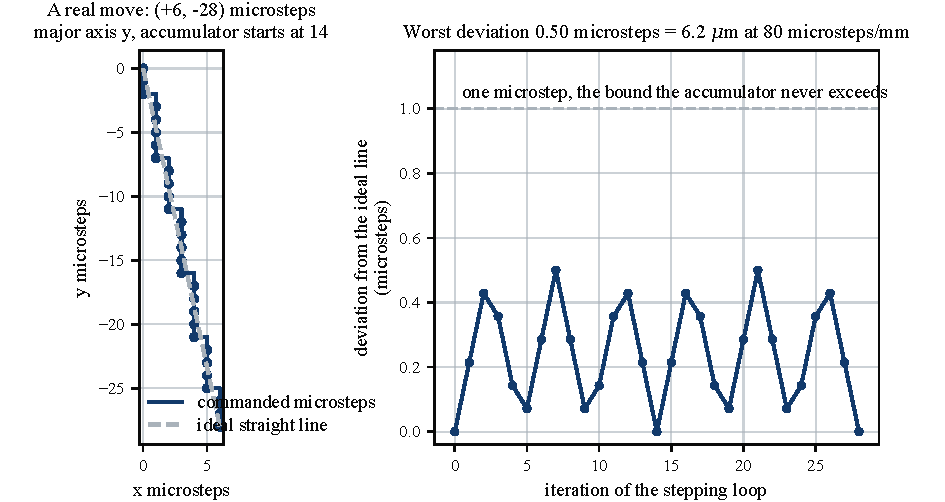
\includegraphics[width=0.96\linewidth]{Figures/VisualTests/T52_bresenham_staircase.pdf}
\caption{Coordinated axis steps and command-space deviation for one generated move.}
\label{fig:vt-stepping}
\end{figure}

The current loop waits inside each axis-pulse call, so an iteration with two pulses waits twice. Its delay contribution is
\begin{equation}
t_{\mathrm{delay}}=(N_M+N_m)\tau,\qquad
\tau=\max\left(\frac{d}{vN_M},2\times10^{-6}\right),\quad v=F/60.
\label{eq:des-pulsetime}
\end{equation}
For the $(3,-29)$ move, $d=0.355373$\,mm and $F=900$\,mm/min give $t_{\mathrm{delay}}=0.02614$\,s, compared with a geometric feed budget of 0.02369\,s. Thus the requested feed is not a measured execution speed; a shared pulse scheduler would reduce this directional timing difference.

Figure~\ref{fig:des-shapetest} compares the G-code preview with the physical square-and-triangle drawing. The 100\,mm square exercises axis-parallel moves, while the triangle's 80\,mm base and two diagonal edges exercise coordinated motion. This checks that the file is interpreted into the intended shapes; the dimensional measurements are reported in Results.

\begin{figure}[!htbp]\centering
\begin{minipage}{0.47\linewidth}\centering
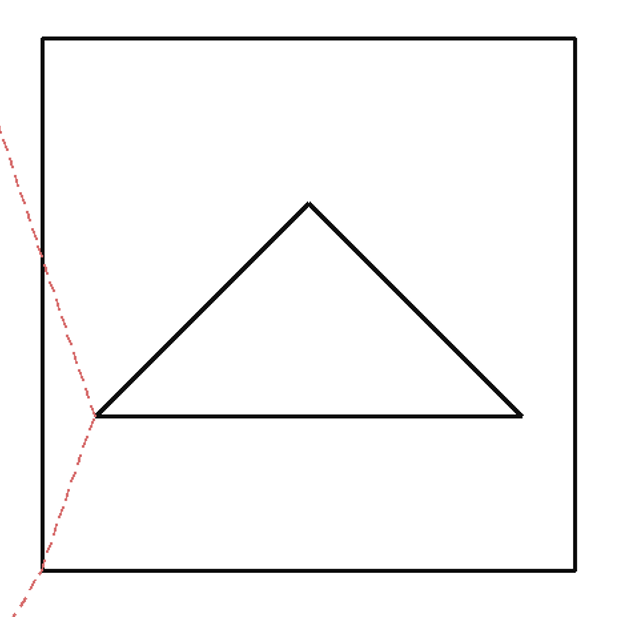
\includegraphics[width=\linewidth,height=0.23\textheight,keepaspectratio]{Figures/square-triangle-gcode-preview.png}\par(a) G-code path preview
\end{minipage}\hfill
\begin{minipage}{0.47\linewidth}\centering
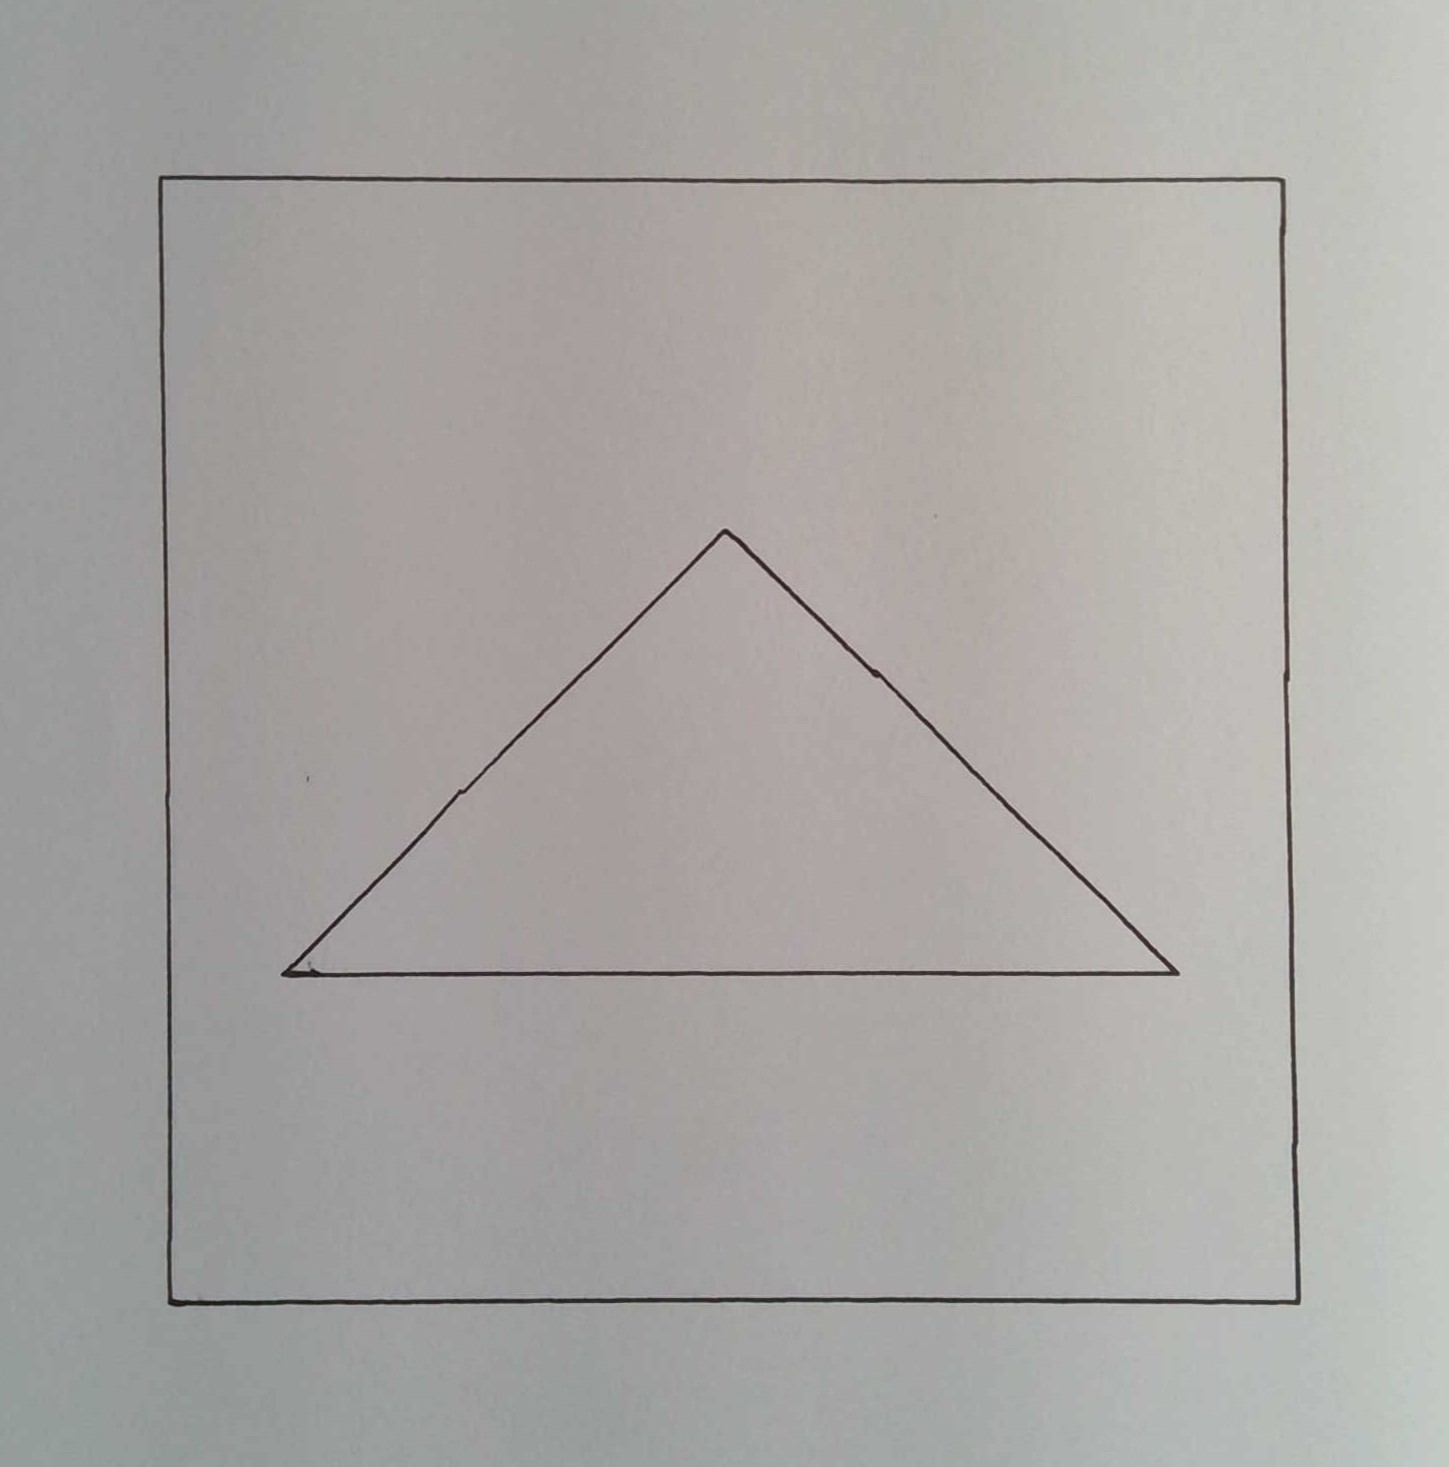
\includegraphics[width=\linewidth,height=0.23\textheight,keepaspectratio]{Figures/square-triangle-reproduced.jpg}\par(b) Physical drawing
\end{minipage}
\caption{G-code preview and the corresponding physical square-and-triangle plot.}
\label{fig:des-shapetest}
\end{figure}
\FloatBarrier
